% !TeX spellcheck = en_US


\chapter{Infrastructure}


\section{Overview}
The system infrastructure facilitates real-time collection, processing, and visualization of sensor data from whisker sensors.
The architecture comprises three main entities: the whisker platform, the controller, and the actuator.
The platform provides two I2C buses for reading sensor data, each equipped with three MLX90393 sensors.
The sensors are connected in a daisy chain via a QUIK connector, enabling solderless connections.
Theoretically, up to 16 sensors can be connected per bus, but in practice, only three are used, as the development boards are limited to four sensors per bus.
The controller is a Raspberry Pi 5 that processes sensor data and generates control signals for the actuator.
Currently, the actuator is simulated; however, it will eventually be replaced by a Franka Emika Panda robotic arm.
Figure~\ref{fig:infrastructure_overview} summarizes the system architecture.

\begin{figure}[htb]
    \centering
    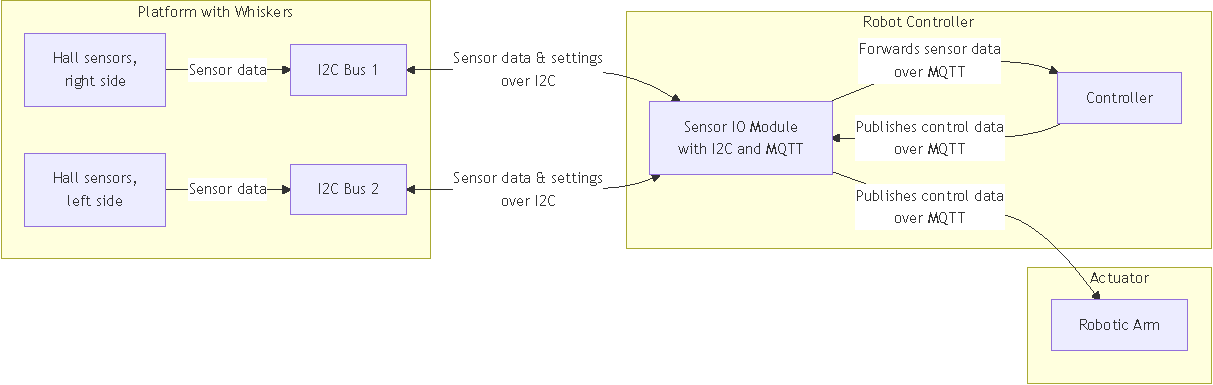
\includegraphics[width=\textwidth]{figures/diagrams/infrastructure-overview}
    \caption{Overview of the system infrastructure.}
    \label{fig:infrastructure_overview}
\end{figure}


\section{Controller}
The control loop of the system is depicted in Figure~\ref{fig:control-flow}.
This loop continuously processes sensor data, evaluates control policies, and generates control messages.
Figure~\ref{fig:control-hierarchy} details the hierarchy of components within the controller.

\begin{figure}
    \centering
    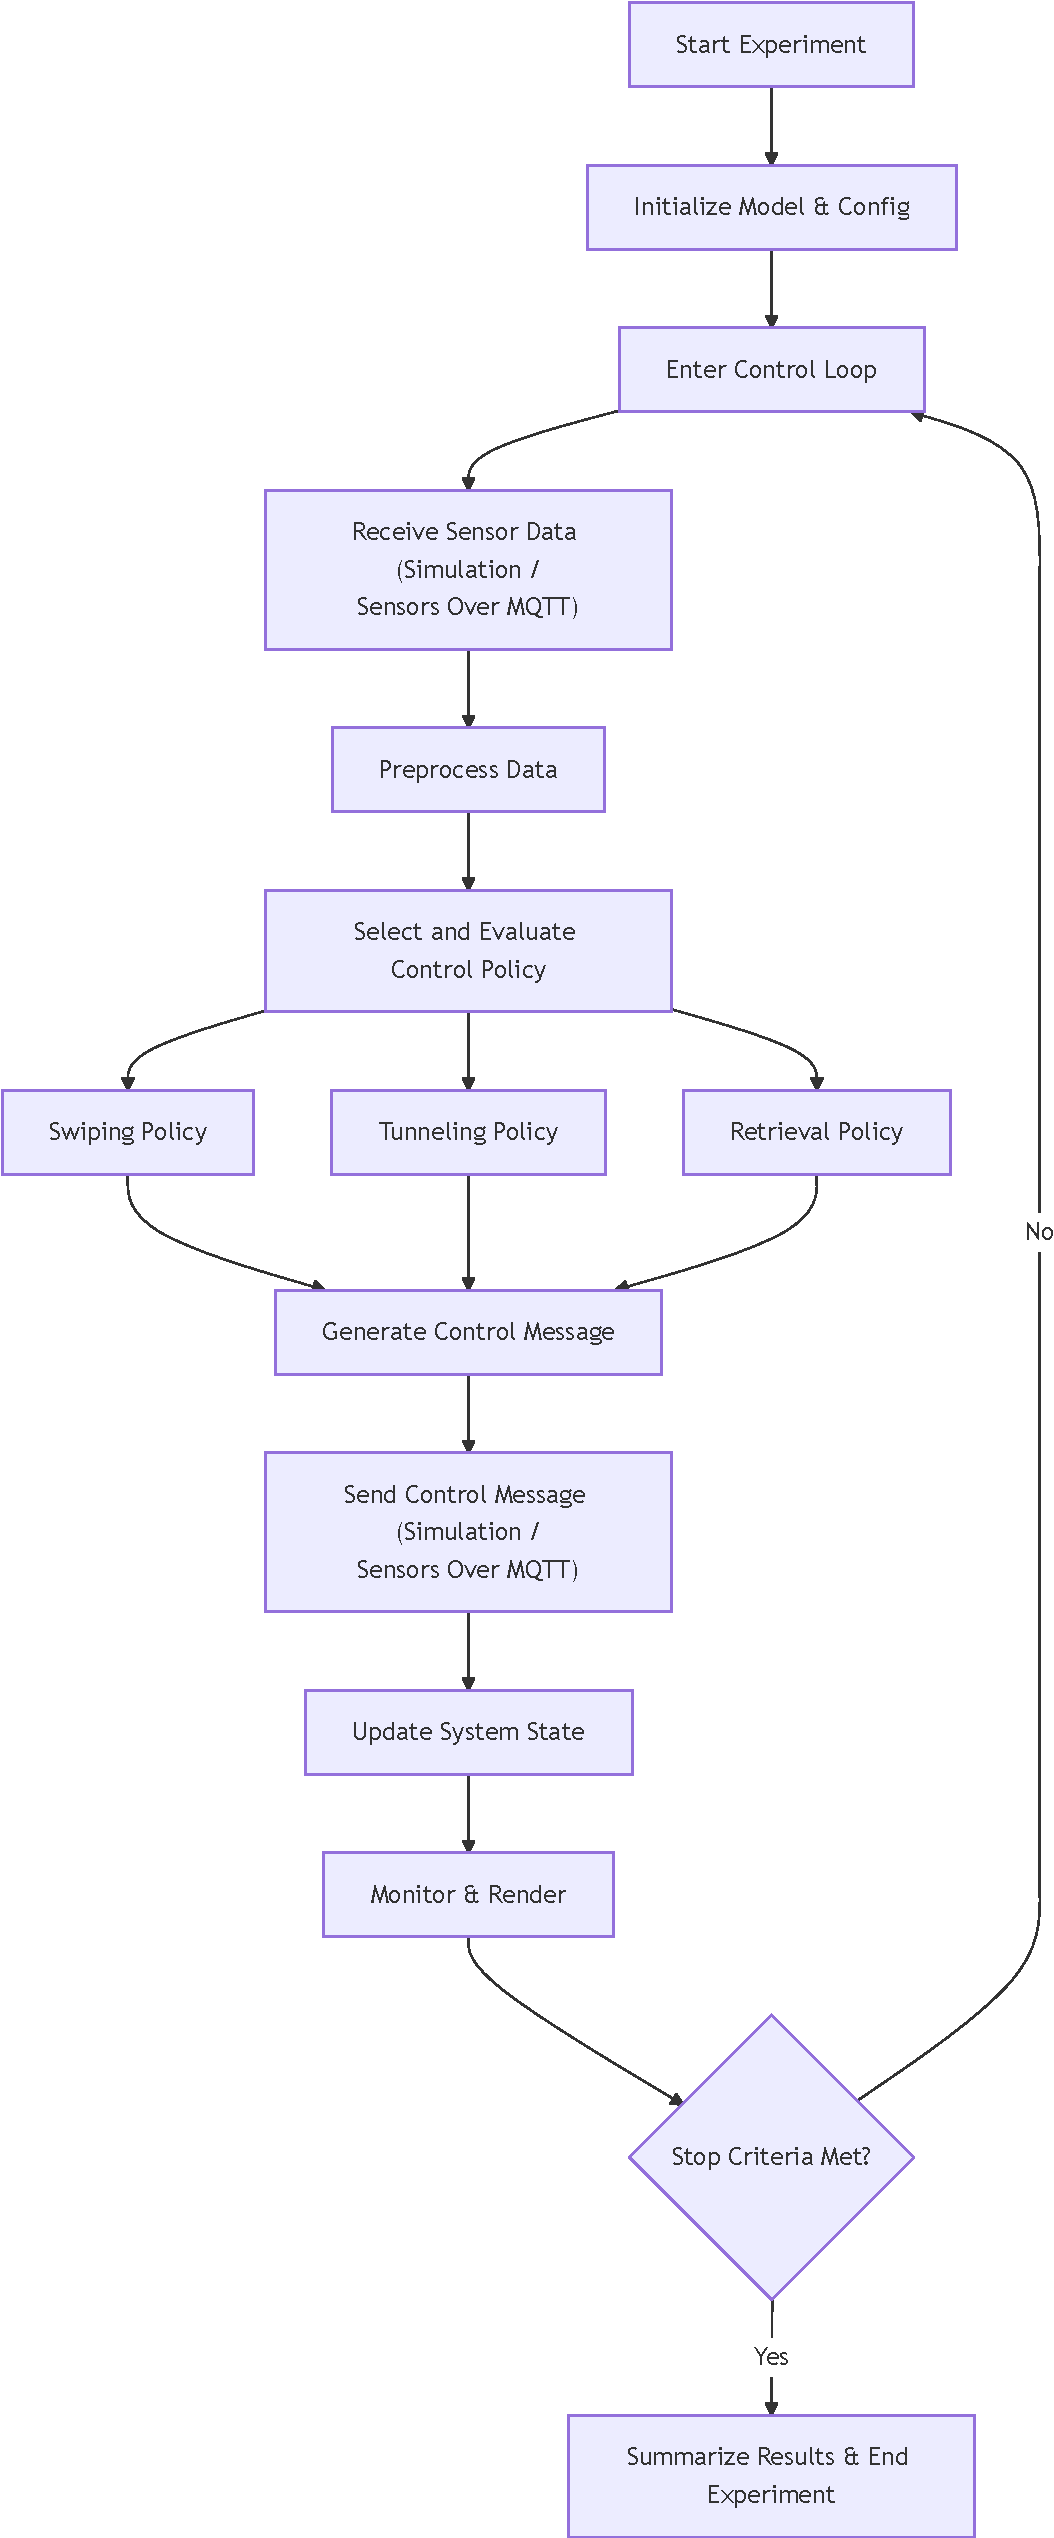
\includegraphics[height=\textheight]{figures/diagrams/control-flow}
    \caption{Data flow in the system infrastructure.}
    \label{fig:control-flow}
\end{figure}


\section{Simulation}
The simulation framework is used for testing the controller.
It provides a realistic physics engine environment for validating control algorithms.
The simulation is based on MuJoCo, a physics engine developed by Google DeepMind.
The interface looks like this~\cref{fig:mujoco}.

\begin{figure}
    \centering
    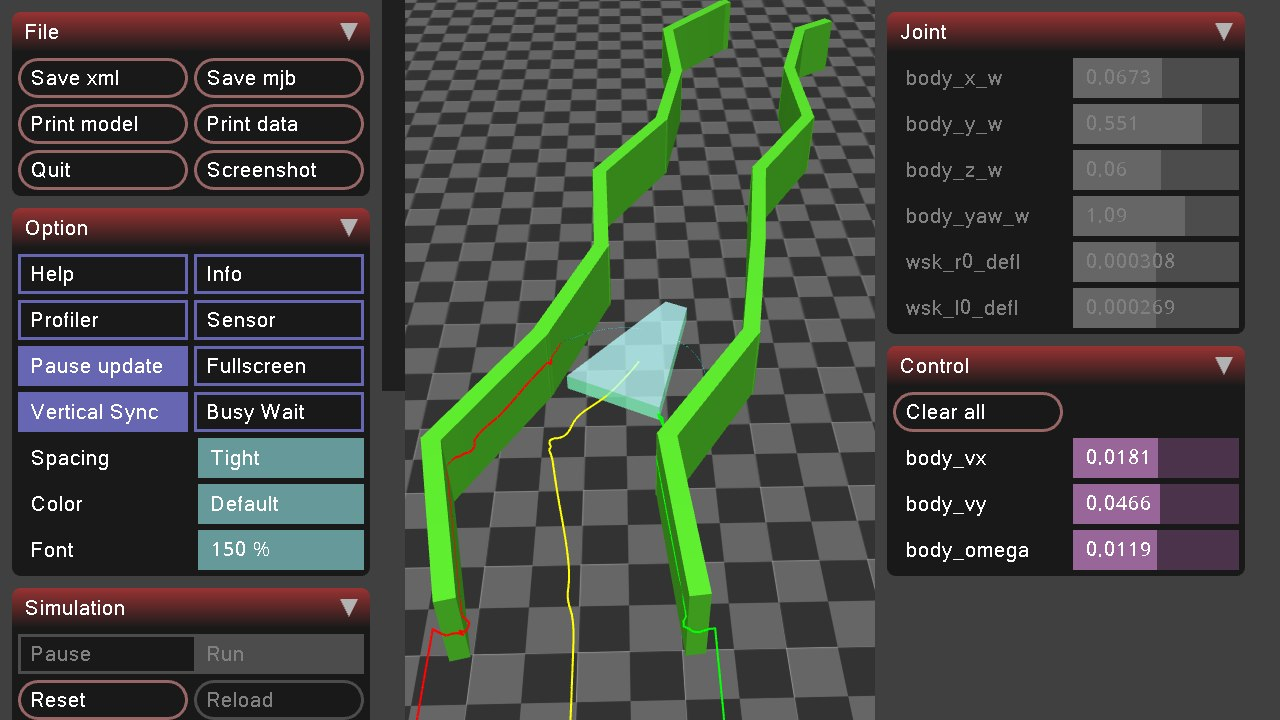
\includegraphics[width=\textwidth]{figures/mujoco}
    \caption{Simulation interface of the MuJoCo physics engine.}
    \label{fig:mujoco}
\end{figure}

The simulation framework is designed to be modular, allowing for easy integration of new components and algorithms.
10 test cases are provided to evaluate the performance of different policies.
Each test case automatically evaluates and plots the results, like in Figures~\ref{fig:experiment-disk-swiping}--\ref{fig:experiment-round-tunnel-swiping-tunneling}.
The controller has no dependency on the simulation framework, allowing for easy integration with other systems.


\section{System Services}
The overall system is composed of several interconnected services that enable robust real-time data exchange.
Figure~\ref{fig:data_flow} illustrates the data flow across these services.
All of those services are running in Docker containers, which allows for easy deployment and management.
They are orchestrated using Docker Compose, which simplifies the setup and configuration of the entire system.
It can run on any machine with Docker installed, like Raspberry Pi 5, making it easy to deploy.

\begin{figure}
    \centering
    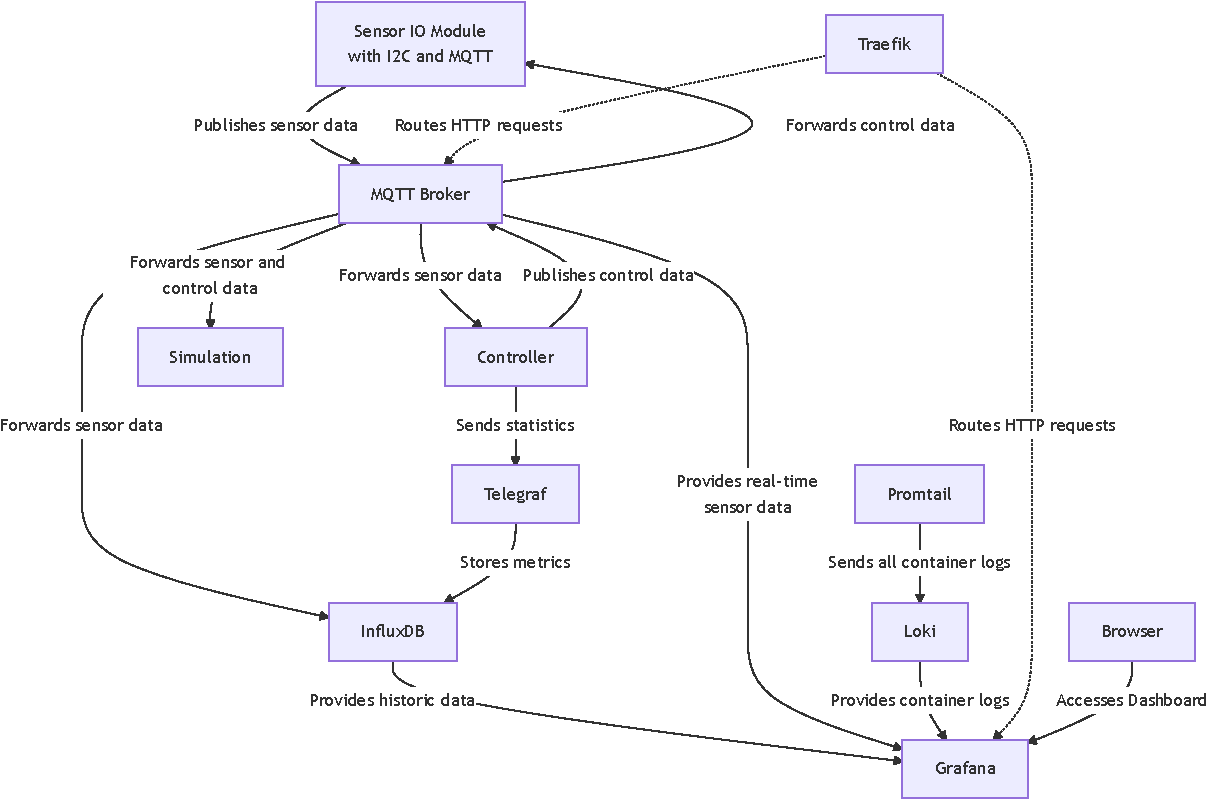
\includegraphics[width=\textwidth]{figures/diagrams/infrastructure-robot-controller}
    \caption{Data flow in the system infrastructure.}
    \label{fig:data_flow}
\end{figure}

\begin{itemize}
    \item \textbf{Sensor IO Module:}
    This module reads sensor data from the robot's I2C buses and publishes the data via MQTT.
    It also forwards control commands from the controller to the actuator.
    Currently, it is embedded in the Raspberry Pi.

    \item \textbf{Controller:}
    The Controller processes sensor data and generates control signals.
    It also publishes statistics for further monitoring.

    \item \textbf{MQTT Broker:}
    Acting as the central messaging hub, the MQTT Broker receives and distributes sensor and control data.
    It is based on the subscriber-publisher model.
    This component is critical for system responsiveness.

    \item \textbf{Telegraf:}
    Telegraf collects sensor data and controller performance metrics.
    The data is then forwarded to InfluxDB for storage.

    \item \textbf{InfluxDB:}
    InfluxDB is a time-series database, which is used to store historical sensor data and controller performance metrics.
    It serves as a persistent storage solution for the system during the execution of the experiments.

    \item \textbf{Grafana:}
    Grafana provides a web-based dashboard that visualizes the sensor data in real-time.
    It allows users to monitor the system's status interactively.

    \item \textbf{Promtail:}
    Promtail is responsible for collecting logs from the various services and forwarding them to Loki.

    \item \textbf{Loki:}
    Loki aggregates the logs provided by Promtail and makes them available for visualization via Grafana.
    This centralized logging system helps in troubleshooting and monitoring system health.

    \item \textbf{Traefik:}
    Traefik is used as a reverse proxy for communication between the services and with the outside world.
    For instance, it allows access to the Grafana dashboard via a web browser.
\end{itemize}


\section{Dashboard}
The system dashboard is built using Grafana, a powerful analytics and monitoring platform.
It provides a web-based interface for visualizing real-time sensor data and control signals.
Grafana Live with MQTT supports real-time monitoring of system status.
Figure~\ref{fig:grafana} shows a barebone dashboard displaying magnetic data from six whisker sensors.


\begin{figure}[htb]
    \centering
    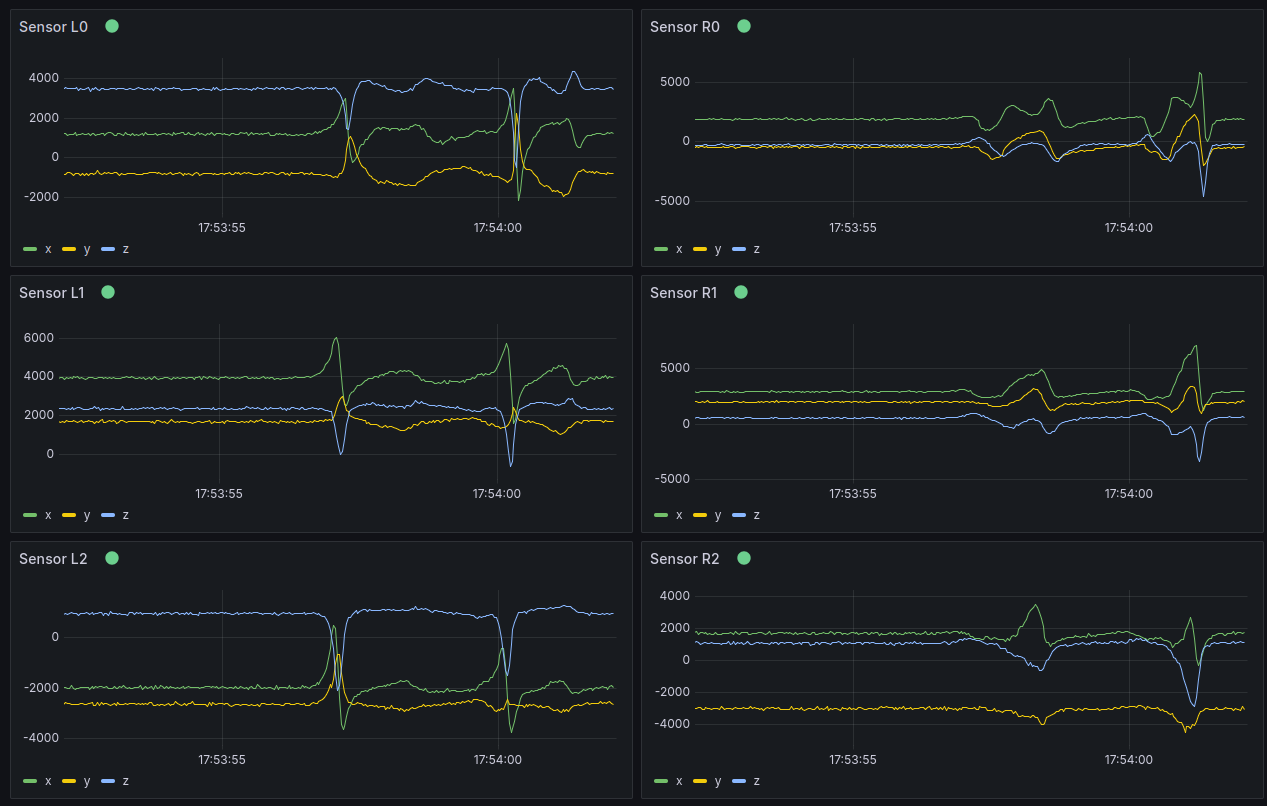
\includegraphics[width=\textwidth]{figures/grafana}
    \caption{Visualization of magnetic data of 6 whisker sensors in real time using Grafana.}
    \label{fig:grafana}
\end{figure}

The plans for the dashboard include:
\begin{itemize}
    \item Visualization of whisker deflection in 2D
    \item State machine visualization
    \item Performance metrics of the contour reconstruction algorithm
    \item System cycle time and overload monitoring
    \item Historical data analysis and trend monitoring.
\end{itemize}

\subsection{MLX90393 Sensor Drivers}
Two MLX90393 sensor drivers have been implemented: one in C++ for the ESP32 microcontroller and another in Python for the Raspberry Pi.
Both drivers provide an API for sensor data acquisition and configuration.
In continuous reading mode, the sensor operates with a high sampling rate.
While up to 16 sensors can theoretically be connected per I2C bus, hardware limitations restrict each bus to four sensors.
This can be overcome by using a custom PCB with chips configured with unique addresses.
